\chapter{Hardware realization of matchers} \label{ch:hdlgen}
We build \gls{rgx} matchers as terms within Gallina, the functional
programming language of Coq.
This chapter describes how Gallina terms are converted to hardware
implementations.
% We need the \gls{rgx} matcher built within Coq to be transformed into
% a hardware implementation.
%
While Gallina offers a high level of abstraction and is suitable for
building proofs within Coq, programs written in it cannot directly be
converted to hardware descriptions.
Hence, we need a way to bridge the gap between the worlds of Gallina
and hardware.
We do this in three stages.
%
\begin{itemize}
  \item Extract \gls{NFA} from Coq to Haskell.
  \item Compile the resultant Haskell code to a Verilog description.
  \item Use \gls{EDA} tools to convert Verilog into an \gls{FPGA}
    loadable bitstream.
\end{itemize}

%% In this chapter, we describe how we use the extraction feature of Coq
%% and the Clash compiler to convert Gallina terms to \gls{HDL}.

%% In the last Chapter, we saw how an \gls{NFA} corresponding to a given
%% \gls{rgx} is generated within Coq. 
%% The \gls{NFA} thus produced are terms in Gallina, the functional
%% programming language of Coq.
%% While Gallina offers a high level of abstraction and is suitable for
%% building proofs within Coq, programs written in it cannot directly be
%% converted to hardware descriptions.
% to convert Gallina to 
% In this chapter we show how the \glspl{NFA} built within Coq are
% converted to corresponding hardware.

% \section{Hardware designs}
% The \gls{NFA} that we construct using Thompson's algorithm as
% described in Section~\ref{sec:nfacon-set} 

\section{Hardware Description Languages}
% Clash is a high-level \gls{HDL} whose syntax very closely resembles
% that of Haskell.
General purpose programming languages commonly used to develop
software are not suitable for expressing hardware designs.
There are inherent differences in the design models of hardware and
software.
% Unlike software, behaviour of hardware is inherently parallel in
% nature and the amount of resources available in a hardware design
% cannot change while it is running.
%
Each component in a hardware circuit is always active and capable of
operating independent of other components.
A language for expressing hardware designs must make it convenient to
indicate how different components of a circuit run and interact.
%
Hence, hardware designs are usually expressed using a special class of
languages known as \glspl{HDL}.
% which are specifically meant for expressing hardware designs.
These languages provide constructs that make it convenient to express
hardware circuits.
%
Although there are numerous \glspl{HDL} available, most hardware
designs in the industry are written in VHDL or Verilog.
The prominence of these two \glspl{HDL} is such that most synthesis
tools expect their input design to be in one of these languages.

\subsection{Synthesizable hardware designs} \label{sec:synthesizability}
% Hardware designs are usually written in a \gls{HDL}.
% In addition to being a means for describing hardware designs,
% \glspl{HDL} also provides extra features that are helpful for
% performing simulation and testing.
% However, these extra features cannot be used 
% %
% In addition to serving as a means for describing hardware designs, \glspl{HDL}

Although the primary use of \glspl{HDL} is to describe hardware
designs, they are also used to facilitate the simulation and testing
of the designs written in them.
This means that in addition to the constructs that can be mapped to
actual hardware, most \glspl{HDL} also offer features that have no
counterparts in hardware.
%
% This makes \glspl{HDL} more restrictive than the languages used to
% build software.
%
For example, it is possible to write \code{for} loops in Verilog.
However, such loops will be fully unrolled before they are processed.
This means that infinite loops cannot be used for designs intended for
synthesis.
Unlike software, the amount of resources available in hardware designs
cannot change while they are running.
%
%% General purpose programming languages offers many constructs which
%% have no counterparts in hardware.
% \section{Function table}
% Not all constructs available in general purpose programming languages
% have counterparts in the hardware world.
% For example, infinite recursion has no counterpart in hardware.
%% For example, recursive functions without a base case cannot be
%% translated to hardware elements.
\glspl{HDL} offer constructs which cannot be mapped to hardware
because such features are useful in writing testbenches.
Such features include directives to initialize registers with set
values and displaying contents of a register.
The features of an \gls{HDL} that can be mapped to actual hardware
components are collectively known as the \emph{synthesizable subset}
of that \gls{HDL}.
% These features are part of the \emph{non-synthesizable subset} of the
% \gls{HDL}.
The design of a hardware circuit should make clear the amount of
resources that is needed in order to synthesize it.
As the use of non-synthesizable features makes this impossible,
hardware designers should limit themselves to the use of the
synthesizable subset of \glspl{HDL} for hardware designs meant for
synthesis.
This is an important consideration in the design of hardware.
%
% As general purpose programming languages are not suited for this
% purpose,
%% Therefore, hardware designs are usually written using \glspl{HDL},
%% which are a special class of languages specifically meant for
%% expressing hardware designs.
%% Hardware designs are usually expressed in an \gls{HDL}.
%% VHDL, Verilog or their variants are the most popular ones used for the
%% purpose.

% The alphabet of the \glspl{NFA} that we saw earlier are in terms of 
% The state of the \gls{NFA}

\subsection{Functional programming for hardware}

%% Despite their overwhelming popularity, neither VHDL nor Verilog were
%% intended for use in synthesis.
Despite the widespread use of VHDL and Verilog to express designs for
synthesis, neither language was designed with hardware synthesis in
mind.
%% be 
%% intended for use in synthesis.
VHDL was originally meant for documenting designs, whereas Verilog was
intended to be used only for simulation purposes.
%% Since both languages ended up being used for 
%
%% Some of these languages were originally meant to be used only for
%% writing specifications and was not intended to be used as input for
%% hardware synthesis.
As a result, the designer often has to work at a lower level of
abstraction than necessary due to the unavailability of richer features.
%
This led to the development of other \glspl{HDL} in which it is more
convenient to write designs.
%
%% Various other \glspl{HDL} have been created to allow designs to be
%% expressed at a higher abstraction level.
%% Among these langauges
%% As functional programming paradigms are suited for expressing
%% hardware~\cite{elliott2017compiling}, many of these languages allow
%% designs to be written as functions.


Functional programming is suited for expressing
hardware~\cite{elliott2017compiling}.
%% The concurrent working of hardware components making functional programming
%% languages well suited for expressing
%% hardware designs~\cite{elliott2017compiling}.
This is because pure functions correspond to combinational hardware
circuits.
Hardware components can be thought of as functions where the input and
output signals correspond to the function arguments and its return
value, respectively.
%
The values present in these signals are tuples if there is more than
one input and output wires.
%% The return value is a multi-element tuple if there is more than one
%% output signal.
Representation of a hardware component with 3 input signals ($a$, $b$,
$c$) and two output signals ($x$, $y$) is shown in
Fig~\ref{fig:hw-fn}.
%% This component can be modeled as a function \code{f :: a -> b -> c ->
%%   (x, y)}, which is a 3-input function returning a 2-element tuple.
This component can be modeled as a function $f$ that accepts the
3-element tuple $(a, b, c)$ to return a 2-element tuple.
  %% (x, y)}, which is a 3-input function returning a 2-element tuple.

\begin{figure}
  \begin{center}
    % \documentclass{article}
% \usepackage{tikz}
% \usetikzlibrary{automata} % Import library for drawing automata
% \usetikzlibrary{positioning} % ...positioning nodes
% \usetikzlibrary{arrows} % ...customizing arrows
% \usetikzlibrary{shapes.misc}
% \usetikzlibrary{arrows.meta,
%                 decorations.markings}



% \usetikzlibrary{decorations.pathreplacing}

% \begin{document}

\begin{tikzpicture}
  \node at (0,0) (inp) {(a, b, c)};
  \coordinate[right of=inp, xshift=1cm] (inp-split);
  \node[right of=inp-split, xshift=1cm,
        draw, fill=gray!20, rectangle,
        minimum width=15mm, minimum height=2cm] (f) {\textbf{f}};
  \coordinate[right of=f, xshift=1.0cm] (out-join);
  \node[right of=out-join, xshift=1cm] (out) {(x, y)};

  \draw (inp.east) to[short,i>=\relax,-*] (inp-split);
  \draw (out-join) to[short,*-]node[currarrow,pos=1]{} (out);
  \draw (inp-split) -- (inp-split|-f.140) to[short,i>=a] (f.140);
  \draw (inp-split) -- (inp-split|-f.220) to[short,i>=c] (f.220);
  \draw (inp-split) to[short,i>=b] (f.west);
  %
  \draw (f.30) to[short,i>=x\relax] (f.30-|out-join) -- (out-join);
  \draw (f.330) to[short,i>=y] (f.330-|out-join) -- (out-join);
\end{tikzpicture}



% \begin{tikzpicture}[
%        ->-/.style = {decoration={markings,
%                                  mark=at position 0.5 with {\arrow{>}}},
%                      postaction={decorate}}
%   ]
%   \node at (0,0) (inp) {(a, b, c)};
%   \node[right of=inp, xshift=1cm] (inp-split) {};
%   \node[right of=inp-split, yshift=0.75cm] (inp-a) {};
%   \node[right of=inp-split] (inp-b) {};
%   \node[right of=inp-split, yshift=-0.75cm] (inp-c) {};
%   \node[right of=inp-b, xshift=-3mm,
%         draw, fill=gray!20, rectangle,
%         minimum width=15mm, minimum height=2cm] (f) {\textbf{f}};
%   \node[right of=inp-b, xshift=0.50cm] (out-b) {};
%   \node[above of=out-b, yshift=-0.50cm] (out-a) {};
%   \node[below of=out-b, yshift=0.50cm] (out-c) {};
%   \node[right of=out-b] (out-join) {};
%   \node[right of=out-join, xshift=1cm] (out) {(x, y)};

%   \fill (inp-split) circle[radius=1pt];
%   \fill (out-join) circle[radius=1pt];
%   \draw[->-] (inp) -- (inp-split);
%   \draw[->] (inp-split) |- (inp-a);
%   \draw[->] (inp-split) |- (inp-b);
%   \draw[->] (inp-split) |- (inp-c);
%   \draw[->] (out-a) -| (out-join);
%   %\draw[->-] (out-b) -- (out-join);
%   \draw[->] (out-c) -| (out-join);
%   \draw[->-] (out-join) -- (out);
% \end{tikzpicture}

% \end{document}

  \end{center}
  \caption{A hardware component as function $f(a, b, c) = (x, y)$}
  \label{fig:hw-fn}
\end{figure}

\section{Clash}
Several \glspl{HDL} have been made that allow hardware designs to be
expressed using functional
programming~\cite{fpinhwsurvey,bachrach2012chisel,ray2023hardcaml}.
%% As functional programming languages are suitable for hardware designs,
%% many \glspl{HDL} have been made which allow writing designs in the
%% functional
%% style~\cite{fpinhwsurvey,bachrach2012chisel,ray2023hardcaml}.
These languages allow designs to be expressed at a higher abstraction level,
resulting in improved expressivity and readability.
One such \gls{HDL} is \emph{Clash}~\cite{clash2010}, a superset of the
Haskell programming language.
The Clash compiler is made by extending the \gls{GHC} with primitives
useful for expressing hardware designs.
This allows designs written in Clash to take advantage of the entire
Haskell ecosystem, including the use of third-party Haskell libraries.
%
The Clash compiler also has a provision that allows us to convert Clash
designs into equivalent VHDL or Verilog/SystemVerilog since most
synthesis tools expect designs to be written in a traditional
\glspl{HDL}.
We take advantage of the ability of the Clash compiler to convert
Haskell code to Verilog, which together with Coq's Haskell extraction
gives us a pathway from Coq to Verilog.
% the Clash compiler also has a provision allowing us to
% convert Clash designs into equivalent VHDL or Verilog/SystemVerilog.
We choose to convert our matchers to Verilog since \gls{FOSS}
synthesis has more support for it.
% The Clash compiler builds on top of GHC and allows conversion of designs
% expressed in Clash to conventional HDLs like VHDL and Verilog.
% Hardware components are expressed as functions.
% One the functions would be marked as the top entity.
% The top entity, together with all definitions used by it, constitutes a
% complete hardware design in Clash.

% A language like Clash has many advantages.
% Clash allows the designer to express ideas at a higher abstraction
% level than is possible with the conventional languages.

% In this work, we extract the matcher model in Coq to Haskell that is
% compatible with Clash.
% Similarity of Clash to Haskell makes it possible for us to use this extracted
% code to construct hardware designs as Clash programs.
% Type classes in Coq are not equivalent to those in Haskell and hence
% Coq-to-Haskell extraction procedure does handles type class instances by adding
% an explicit extra argument.

\subsection{Advantages}
The use of Clash for hardware design offers many advantages over
traditional \glspl{HDL}.
For example, the ability to make user-defined data types can greatly
enhance readability of designs.
We can take advantage of the entire feature set of the \gls{GHC}
compiler while defining types in Clash.
This includes features like generalized algebraic data types (GADT)
which are made available via
%% This includes features like \glspl{GADT} which are made available via
\gls{GHC} extensions.
%% even make use of  feature of Haskell while defining
%% types in Clash.
In the case of languages like SystemVerilog, options to define our own
types are limited to relatively primitive types like enumeration
types, structures and unions.

% Remove: Not true for VHDL. True for Verilog though.
The weak typing of Verilog means that the designer has to be aware of
the size of the values at each point to avoid surprises during
simulation.
In contrast, Clash can automatically figure out the size required for
types that it knows to be finite.
A trivial example is shown in Fig~\ref{code:type-strength}, where
assignment of a value with a type different than what was declared
produces error in Clash, but not in Verilog.
%% Being a strongly typed langauge, VHDL is strongly typed, but it requires designs to be expressed at a
%% lower abstraction level.
%
%% Any type that is definable in standard Haskell is also definable in
%% Clash.
%% However, only finite types can be used for a synthesizable
%% design (see Section~\ref{sec:synthesizability}).
%% Even the extra features offered by GHC extensions and third party
%% Haskell packages can be utilized.
%
%% Type system of a language like Haskell/Clash is much more powerful
%% than that of Verilog.
Clash also allows us to express polymorphic designs.
i.e., the same function can be used with different values to produce
different designs.
%% This is possible towards a certain extent with VHDL's generics as
%% well.

%% \begin{table}
%%   \centering
%%   \begin{tabular}{ll}
%%     \toprule
%%     Type                & Size                    \\
%%     \midrule                                 
%%     \code{()}           & 1                       \\
%%     \code{Bool}         & 2                       \\
%%     \code{Either t1 t2} & max(size(t1), size(t2)) \\
%%     \code{(t1, t2)}     & size(t1) + size(t2)     \\
%%     \bottomrule
%%   \end{tabular}
%%   \caption{Size of finite types in Haskell}
%%   \label{tab:type-sizes}
%% \end{table}

\begin{figure}
  \begin{minipage}{0.5\textwidth}
    \begin{Verbatim}[commandchars=\\\{\}]
\PY{k}{module}\PY{+w}{ }\PY{n}{typerr}\PY{+w}{ }\PY{p}{(}
\PY{+w}{    }\PY{k}{input}\PY{+w}{ }\PY{p}{[}\PY{l+m+mh}{2}\PY{o}{:}\PY{l+m+mh}{0}\PY{p}{]}\PY{+w}{ }\PY{n}{x}\PY{p}{,}
\PY{+w}{    }\PY{k}{output}\PY{+w}{ }\PY{n}{msb}
\PY{p}{)}\PY{p}{;}

\PY{+w}{  }\PY{k+kt}{wire}\PY{+w}{ }\PY{p}{[}\PY{l+m+mh}{1}\PY{o}{:}\PY{l+m+mh}{0}\PY{p}{]}\PY{+w}{ }\PY{n}{less}\PY{p}{;}
\PY{+w}{  }\PY{k+kt}{wire}\PY{+w}{ }\PY{p}{[}\PY{l+m+mh}{3}\PY{o}{:}\PY{l+m+mh}{0}\PY{p}{]}\PY{+w}{ }\PY{n}{more}\PY{p}{;}

\PY{+w}{  }\PY{c+c1}{// No error}
\PY{+w}{  }\PY{k}{assign}\PY{+w}{ }\PY{n}{less}\PY{+w}{ }\PY{o}{=}\PY{+w}{ }\PY{n}{x}\PY{p}{;}
\PY{+w}{  }\PY{k}{assign}\PY{+w}{ }\PY{n}{more}\PY{+w}{ }\PY{o}{=}\PY{+w}{ }\PY{n}{x}\PY{p}{;}
\PY{k}{endmodule}
\end{Verbatim}

  \end{minipage}
  \begin{minipage}{0.5\textwidth}
    \begin{Verbatim}[commandchars=\\\{\}]
\PY{n+nf}{x}\PY{+w}{ }\PY{o+ow}{::}\PY{+w}{ }\PY{k+kt}{Vec}\PY{+w}{ }\PY{l+m+mi}{3}\PY{+w}{ }\PY{k+kt}{Bool}
\PY{n+nf}{x}\PY{+w}{ }\PY{o+ow}{=}\PY{+w}{ }\PY{k+kt}{True}\PY{+w}{ }\PY{k+kt}{:\PYZgt{}}\PY{+w}{ }\PY{k+kt}{False}\PY{+w}{ }\PY{k+kt}{:\PYZgt{}}\PY{+w}{ }\PY{k+kt}{True}\PY{+w}{ }\PY{k+kt}{:\PYZgt{}}\PY{+w}{ }\PY{k+kt}{Nil}

\PY{c+c1}{\PYZhy{}\PYZhy{} Error}
\PY{n+nf}{less}\PY{+w}{ }\PY{o+ow}{::}\PY{+w}{ }\PY{k+kt}{Vec}\PY{+w}{ }\PY{l+m+mi}{2}\PY{+w}{ }\PY{k+kt}{Bool}
\PY{n+nf}{less}\PY{+w}{ }\PY{o+ow}{=}\PY{+w}{ }\PY{n}{x}

\PY{c+c1}{\PYZhy{}\PYZhy{} Error}
\PY{n+nf}{more}\PY{+w}{ }\PY{o+ow}{::}\PY{+w}{ }\PY{k+kt}{Vec}\PY{+w}{ }\PY{l+m+mi}{4}\PY{+w}{ }\PY{k+kt}{Bool}
\PY{n+nf}{more}\PY{+w}{ }\PY{o+ow}{=}\PY{+w}{ }\PY{n}{x}
\end{Verbatim}

  \end{minipage}
  \caption{A difference between type systems of Verilog and Clash}
  \label{code:type-strength}
\end{figure}


Another advantage of designs written in Clash is that simulation can
be performed within a \gls{REPL}.
This is much more convenient than what is the case for Verilog, where
test benches have to be written, simulated and then wave forms
examined in order to test and debug designs.
The use of a \gls{REPL} allows for rapid prototyping and testing.
In addition, test benches written in Clash can be converted to Verilog.

% \begin{itemize}
% \item Readable code. User defined types.
% \item Powerful type system % verilog allows 3b assignment to a 5b wire
% \item Polymorphism. Only top-level components need to be instantiated
% \item
%   Simulation possible within Haskell \gls{REPL}.
%   No need of boilerplate associated with testbenches.
% \end{itemize}

% When compared to traditional \glspl{HDL} like Verilog and VHDL, Clash
% offers many advantages. This includes:

% \begin{itemize}
%   \item Concise, readable code
%   \item Easier simulation within a REPL
%   \item Powerful and expressive type system
%   \item Full utility of Haskell ecosystem
% \end{itemize}

\subsection{Disadvantages}
Despite the many advantages of using Clash for expressing hardware
designs, it is not without a few disadvantages of its own.
This is mainly because its user base is much smaller than that of the
traditional \glspl{HDL} and hence the amount of work that goes into
improving the Clash ecosystem is much lesser.
For example, results from a Clash simulation cannot readily be viewed
as waveforms as Clash does not come with facilities for the same.
This may be due to the comfort offered by \gls{REPL}-based
simulation, making waveform viewing less necessary.
Clash can still dump data that can be used by waveform viewing tools.

One of the drawbacks of using Clash is that it is difficult to
incorporate existing designs and \gls{IP}-blocks.
%% It is difficult to incorporate designs written in other languages like
%% Verilog in a Clash design.
A problem on the other side of the fence is that in order for a Clash
design to be used in a Verilog design, the Clash design first needs to
be converted to Verilog.
However, as the generated code is not very readable, it is difficult
to debug errors that may arise during the integration of designs.
%Though simulation is more convenient with clash designs the waveforms from the
%simulation cannot be viewed from 1 cannot
% https://hackage.haskell.org/package/clash-prelude-1.8.1/docs/Clash-Prelude.html#g:16

Functional programming languages have a reputation for having a
steep learning curve.
This is a significant reason behind the lack of adoption of languages
like Clash in hardware design.
The popularity of Bluespec SystemVerilog in comparison with the
Haskell-like Bluespec Classic illustrates this point.
Veteran \gls{EDA} practitioners may find less incentive in embracing a
less established language that uses a functional programming style for
designs.

Though Clash allows us to work from a higher abstraction level, it can
also hinder the designer from having a fine-grained control over the
design if needed.
For example, precise control over control timing behaviour is
difficult to achieve from within Clash.
% like clock domain crossing.
The need for such control while still maintaining a relatively high
level of abstraction is an active area of
research~\cite{nigam2023modular}.
% Filament

% \begin{itemize}
% \item Generated VHDL/Verilog is difficult to understand
% \item Difficult to incorporate pre-existing \gls{IP} blocks
% \item Lack of supporting tools like waveform viewer
% \item Established \gls{EDA} designers are often not familiar with syntax % Example Bluespec classic
% \item Difficult control timing behaviour. Eg: Clock domain crossing
% \item Extra compilation step when converting VHDL/Verilog
% \end{itemize}
%
%Despite, their many advantages, industry has been reluctant to adopt these
%languages.

\subsection{The \code{mealy} function}
The standard library of Clash offers a function named \code{mealy}
(Fig.~\ref{code:mealy-function}) which can be used to build hardware
descriptions of Mealy machines within Clash.
We use this function to build Clash designs of our \gls{rgx} matchers.
%
%% Given the  corresponding to a \gls{DFA}, given
%% information regarding its transition function, initial state 
%% and the output function.
Given the information regarding the transition function, initial state
and the output function of an automaton, \code{mealy} can produce a
design complete with clock, reset and enable signals.
%
%% In addition to input and output signals, the design so created would
%% have clock, reset and enable signals.
In our case, the output function can be made as a simple check to see
if the set of current states and the set of final states have any
overlap.
The \code{mealy} function, together with the \code{trans} field of the
\code{nfa} type can be used to make the first argument to be passed
onto \code{mealy} function.
The remaining argument is readily available as the \code{start} field
of the \code{nfa} value.

\begin{figure}
  \begin{Verbatim}[commandchars=\\\{\}]
\PY{n+nf}{mealy}
\PY{+w}{  }\PY{o+ow}{::}\PY{+w}{ }\PY{p}{(}\PY{k+kt}{HiddenClockResetEnable}\PY{+w}{ }\PY{n}{dom}\PY{p}{,}\PY{+w}{ }\PY{k+kt}{NFDataX}\PY{+w}{ }\PY{n}{state}\PY{p}{)}
\PY{+w}{  }\PY{o+ow}{=\PYZgt{}}\PY{+w}{ }\PY{p}{(}\PY{n}{state}\PY{+w}{ }\PY{o+ow}{\PYZhy{}\PYZgt{}}\PY{+w}{ }\PY{n}{input}\PY{+w}{ }\PY{o+ow}{\PYZhy{}\PYZgt{}}\PY{+w}{ }\PY{p}{(}\PY{n}{state}\PY{p}{,}\PY{+w}{ }\PY{n}{output}\PY{p}{)}\PY{p}{)}\PY{+w}{     }\PY{c+c1}{\PYZhy{}\PYZhy{} Transition function}
\PY{+w}{  }\PY{o+ow}{\PYZhy{}\PYZgt{}}\PY{+w}{ }\PY{n}{state}\PY{+w}{                                   }\PY{c+c1}{\PYZhy{}\PYZhy{} Initial state}
\PY{+w}{  }\PY{o+ow}{\PYZhy{}\PYZgt{}}\PY{+w}{ }\PY{k+kt}{Signal}\PY{+w}{ }\PY{n}{dom}\PY{+w}{ }\PY{n}{input}\PY{+w}{                        }\PY{c+c1}{\PYZhy{}\PYZhy{} Input}
\PY{+w}{  }\PY{o+ow}{\PYZhy{}\PYZgt{}}\PY{+w}{ }\PY{k+kt}{Signal}\PY{+w}{ }\PY{n}{dom}\PY{+w}{ }\PY{n}{output}\PY{+w}{                       }\PY{c+c1}{\PYZhy{}\PYZhy{} Output}
\end{Verbatim}

  \caption{\code{mealy} function of Clash}
  \label{code:mealy-function}
\end{figure}

% Similar to the concept of synthesizable subset in other \glspl{HDL}
% like Verilog, Clash places certain constraints for designs meant for
% synthesis.
% For example, the \code{mealy} type shown in
% Fig.~\ref{code:mealy-function} imposes the class constraint
% \code{NFDataX} on the type representing the automata states.
% This constraint is imposed to ensure that the state is always a value
% that can be stored in a hardware register.
% %
% %% Clash imposes certain constraints on the type representing the state
% %% of the Mealy machine as the state should be a value which will be
% %% stored in a register.
% It essentially means that the state type should be a finite type.
% % The size of the values of a finite type would be known at compile
% % time.
% However, the Clash compiler is not always capable of recognizing that
% a given user defined type is finite.
% %
% %% Although it is sometimes possible to automatically derive
% %% \code{NFDataX} instances for simple types
% %
% % But as the \code{Vec} type indicative of vectors is already recognized
% % by Clash to be a finite type, we represent the state space of the
% Apart from the computation friendly nature of \code{func}, this is
% another reason why we used \code{func} to indicate states in our
% \code{nfa} type.
% % These values are readily converted to \code{Vector.t}, which after
% % extraction can be mapped to the \code{Vec} type of Clash standard
% % library.
% %
% % This means that the Clash compiler can figure out the maximum 
% % the size of whose part of the Clash standard library, 
% % explicit the finiteness of the type used to denote the state space of
% % the automata.
% %
% The \code{func} fields of a given \code{nfa} value are flattened to
% produce corresponding \code{Vector.t} values before they are extracted
% out of Coq.
% The \code{Vector.t} type is the vector type that is part of the Coq
% standard library.
% The structure of this type is similar to that of the primitive vector
% type of Clash, namely the \code{Vec} type.
% %% Being a primitive type of Clash, the Clash compiler is already aware
% %% that \code{Vec} has an \code{NFDataX} instance.
% This makes it possible for the Coq extraction procedure to convert the
% \code{func} values to corresponding \code{Vec} values.
% As a result, we obtain the fields of the \code{nfa} value as
% \code{Vec} values, which is the type used in Clash to represent
% vectors.
% %
% Clash would be able to recognize designs made using \code{Vec} as
% finite and synthesizable as this type is already known to the Clash
% compiler to be a finite type.

\section{Extraction of NFA from Coq}
Most synthesis tools expect their input hardware designs to be written
in a traditional \gls{HDL} like VHDL and Verilog.
Thus, we need to convert the \gls{NFA} generated within Coq to the
synthesizable subset of an \gls{HDL} before it can be made into a
hardware implementation.
%% In order to convert the \gls{NFA} generated within Coq to hardware, we
%% need it as a \emph{synthesizable} description in a traditional
%% \gls{HDL}.
%% ie, a description which uses only the \gls{HDL} constructs which can
%% be mapped to hardware.
% \gls{HDL} (like Verilog) that is acceptable to synthesis tools.
For this, we have set up a mechanism
involving the Clash compiler
by which the Gallina terms can automatically be converted into
descriptions of hardware components in Verilog.
% We chose Verilog instead of VHDL as the former is better supported by
% \gls{FOSS} tools for hardware synthesis.

Coq offers a feature called \emph{extraction} by which Gallina
terms constructed within Coq may be converted to values in other
languages.
However, Coq does not support extraction to an \gls{HDL} straight out
of the box.
Only Haskell, OCaml, Scheme and JSON are available by default.
It is possible to write a custom extraction procedure by means of a
Coq plugin, but we opted to not do that as it is difficult to get such
a procedure correct whereas the extraction to languages that are
supported by default is battle-tested.
Instead, we first extract the Coq definition into Haskell and then use
the Clash compiler to convert the resultant Haskell code to Verilog.
%% We chose Verilog over VHDL due to the former having better support in
%% \gls{FOSS} \gls{EDA} tools.
%% a Haskell-like \gls{HDL} whose compiler is capable converting
%% Haskell-like code to \glspl{HDL}, including Verilog.
Thus, we derive the design for the desired \gls{rgx} matcher as a
description in Verilog.
% extract the details of the generated \gls{NFA} to Haskell
% using the default Coq extraction procedure and then use the Clash
% compiler to produce corresponding Verilog.
%
Note that arbitrary Gallina terms are not suitable for conversion to
Verilog.
We want terms in a form that can directly be mapped to synthesizable
\gls{HDL} constructs.
This is why we define \code{nfa} in terms of \code{sort} and
\code{func} types.
These types are engineered in such a way that they can be converted to
Haskell terms which in turn may be converted to synthesizable Verilog.

% Like in the case of other \glspl{HDL}, not every design expressible in
% Clash is synthesizable.
% This is not a limitation of Clash and is due to the nature of hardware
% itself.
% because 


%% \subsection{Coq to Verilog}
We extract the transition function and the set of start and final
states of the \gls{NFA} corresponding to the desired \gls{rgx} matcher
as Haskell from Coq.
Although we construct the \gls{NFA} in terms of the \code{func} type,
we convert the \code{func} values to the corresponding \code{Vector.t}
type just before extraction.
This conversion is done to map \code{func} values from Coq to
corresponding \code{Vec} values in Clash as described in Chapter 3.
% This conversion to a Coq built-in type is done to facilitate mapping
% of \gls{NFA} information to the \code{Vec} type of Clash.
% The \code{Vec} type is a primitive type in Clash whose structure is
% same as that of \code{Vector.t}. 
% Since \code{func} is essentially a more structured form of
% \code{Vector.t}, we can flatten the \code{func} values to produce
% values of the \code{Vector.t} type.

The Haskell code extracted from Coq is made into a module named
\code{Nfadata}.
%% Depending on the size of the input \gls{rgx}, \code{Nfadata} module
%% can span a couple dozen lines to hundreds of thousands of \gls{LOC}.
The Clash code describing how the \gls{NFA} is run is made available
as a pre-written module named \code{Mon}. 
This module makes use of the information from the \code{Nfadata}
module and contains the top level of the overall design.
The \code{Nfadata} and \code{Mon} modules are organized using the
cabal build tool to build a complete Haskell project.
Finally, the Clash compiler is used via cabal to produce the Verilog
counterpart of the Clash design.
A schematic showing the processes involved in the conversion of Coq
code to Verilog is shown in Fig.~\ref{fig:extr2hdl-flow}.

\begin{figure}
  \begin{center}
  \begin{tikzpicture}[
  block/.style = {
    draw,
    shape=rectangle,
    minimum width=1.2cm,
    minimum height=1.2cm,
    fill=gray!20,
    align=center
  },
]
  \node (coq) [block] {Coq};
  \node (nfadata) [right of=coq, xshift=2.75cm] {\texttt{Nfadata.hs}};
  \node (mon) [below of=nfadata] {\texttt{Mon.hs}};
  \node (cabal) [shape=ellipse, draw, right of=nfadata, xshift=1.75cm] {cabal};
  \node (proj) [draw, rectangle, right of=cabal, xshift=2.0cm] {Project};
  \node (hdl) [block] [right of=proj, xshift=2.0cm] {Verilog};

  \draw[->] (coq) -- (nfadata) node[above,midway] {Extract};
  \draw[->] (nfadata) -- (cabal)  {};
  \draw[->] (mon) -| (cabal)  {};
  \draw[->] (cabal) -- (proj) node[above,midway] {Build};
  \draw[->] (proj) -- (hdl) node[above,midway] {Clash};
\end{tikzpicture}


  \end{center}
  \caption{Extraction flow}
  \label{fig:extr2hdl-flow}
\end{figure}

\section{Use of function table} \label{sec:ft-clash}
Recall that we use a function table $ft$ to run the \glspl{NFA} that
we build (see Section~\ref{sec:c3-ft}).
The function table allows us to decouple \gls{NFA} from the
tests that are part of the input \gls{rgx}.
%
This is done to allow the type indicative of the \gls{NFA} state space
to be a type whose values can be reduced to a normal form and hence be
stored in a hardware register.
%
% The usage of $ft$ allows us to decouple the tests present in the input
% \gls{rgx} from the \gls{NFA} representing the corresponding matcher.
%
The function table $ft$ facilitates the proper extraction of the
generated matchers in a form that can be used by the Clash compiler to
produce synthesizable Verilog code.
%
% This is to satisfy certain constraints that Clash imposes on designs
% meant for synthesis.

Similar to the concept of synthesizable subset in \glspl{HDL}
like Verilog, Clash places certain constraints on designs meant for
synthesis.
For example, the \code{mealy} type shown in
Fig.~\ref{code:mealy-function} imposes the constraint \code{NFDataX}
on the type representing the automata states.
% This constraint is imposed to ensure that the state is always a value
% that can be stored in a hardware register.
%
% This function requires the type representing the state space of the
% automata to satisfy certain constraints.
% Among these constraints is the need for the state type to be an
% instance of the \code{NFDataX} type class, which is a way of
% indicating that the values of that type are fit to be stored in
% registers.
% which includes this bein.
%
It essentially means that the state type should be a finite type and
that its values have normal forms.
% The size of the values of a finite type would be known at compile
% time.
%
The alphabet of our input \gls{rgx} are boolean functions.
The state type would have been a function of type $s \to \mathbb{B}$
if the alphabet of the corresponding \gls{NFA} were functions as well.
%
Since the state needs to be stored in a register and functions cannot
be stored in registers, we instead use a \code{sort} as the alphabet
of \code{nfa} values.
% It is difficult to write an \code{NFDataX} instance for functions
This necessitates a need to translate between the alphabet of the
input \gls{rgx} and that of the \gls{NFA}, which is fulfilled by the
function table.


However, the Clash compiler is not always capable of recognizing that
a given user-defined type is finite.
%
% % As described in Section~\ref{} use the 
% We use the \code{mealy} function of Clash to construct our matcher
% designs.
% % using the \gls{NFA} transition information generated within Coq.
% The \code{mealy} function is a convenient way to build a hardware
% design in Clash using the transition function and state information of
% an automata.
%
%
The state type for of our \glspl{NFA} is the \code{func s bool} type.
%
Though \code{func} is a family of finite types, it is difficult to
define an \code{NFDataX} instance for it.
% Though values of \code{func s bool}, being elements of a finite type,
% are capable of being stored in a register, it is not straightforward
% to define an \code{NFDataX} instance for \code{func}.
Instead, we translate \code{func} values into corresponding
\code{Vector.t} values before extraction.
%
Unlike \code{func}, the \code{Vector.t} type has the same structure as
the \code{Vec} type available as part of the standard library of
Clash.
This gives us a way to map \code{func} values directly to \code{Vec}
during extraction, since \code{func} can be trivially converted to
\code{Vector.t}.
Being a built-in type, the \code{Vec} type is already known to the
Clash compiler to be an \code{NFDataX} instance.
Therefore, the translation of \code{func} to \code{Vector.t} right
before extraction lets us get around the need to define an
\code{NFDataX} instance by ourselves.
The function table acts as the link between the \gls{NFA} and the
tests present in the input \gls{rgx}.
% This has the added advantage of being able to use the \oc
% But there is still one problem: the transition function of the
% \gls{NFA} are defined on the basis of the tests in the input
% \gls{rgx}.
% And these tests use the current input symbol as argument.
% The manner in which Gallina terms are reduced means that the term
% corresponding to the next state of the \gls{NFA} would essentially be
% a function depending on future input rather than being a concrete,
% fully reduced \code{func} value.
% The computation to derive the next state stops at the point where a
% future input symbol is required. A representation of this scenario is
% shown in Fig.~\ref{fig:delta-no-ft}.
% As this situation leads to the state value being a function, Clash
% compiler would generate error since such values cannot be stored in
% registers.
% This is because pure functions in Clash represent an entire circuit,
% which cannot be stored in a register.
% We utilize function table to avoid this problem.

% Thus, we keep the test from the input \gls{rgx} separate from the
% \gls{NFA} corresponding to its matcher with the help of the function
% table.

% The function table acts as the link between the \gls{NFA} and the
% tests present in the input \gls{rgx}.
% Use of function table $ft$ allows us to decouple the tests in the
% input \gls{rgx} from the \gls{NFA}.
% This makes the \gls{NFA}'s transition function independent of the
% tests, thus avoiding the suspended computation
% problem.
% Fig.~\ref{fig:delta-yes-ft} depicts the scenario of computing the next
% state when the \gls{NFA} is independent of the tests.
%
%%%%
%
%


\section{FPGA implementation} \label{sec:eda}
Having obtained the Verilog code for our desired matcher from the
Clash compiler, we need to convert it into a form that can be loaded
onto hardware.
There are multiple steps involved in generating an \gls{FPGA} loadable
bitstream corresponding to a given Verilog design.
The Verilog code is first synthesized to a netlist form.  The
different components present in this netlist are mapped to the
resources available in the target \gls{FPGA} via a process known as
placement.
Another process called routing connects the placed components
together.
Finally, the resultant design is converted into a bitstream format
compatible with the target \gls{FPGA}.
All these steps can be performed using an \gls{EDA} toolchain.
Though both proprietary and open source \gls{EDA} tools are available,
we use \gls{FOSS} tools to leave more room for possible future
modifications.

We target a Gowin LittleBee \gls{FPGA} whose bitstream format is
documented by Project Apicula~\cite{projapicula}.
Fig~\ref{fig:eda-flow} shows the pipeline that we use to convert
the Verilog design into a bitstream that can be loaded onto
\gls{FPGA}.
%
We use Yosys~\cite{wolf2013yosys} to synthesize the Verilog design
into a netlist. This netlist is used by nextpnr~\cite{shah2019yosys}
to perform placement and routing with respect to the target
\gls{FPGA}.
nextpnr also performs \gls{STA}.
The bitstream for the \gls{FPGA} is generated using a tool from
Project Apicula, and the generated bitstream is finally loaded onto
\gls{FPGA} with the openFPGALoader~\cite{Tang2019openFPGA} tool.
Thus, we achieve a complete flow from the input \gls{rgx} to an
\gls{FPGA} bitstream.
The versions of the tools that we used for our experiments are shown
in Table~\ref{tab:tool-versions}.
  
\begin{figure}
  \begin{center}
  % \documentclass{article}
% \usepackage{tikz}
% \usetikzlibrary{automata} % Import library for drawing automata
% \usetikzlibrary{positioning} % ...positioning nodes
% \usetikzlibrary{arrows} % ...customizing arrows
% \usetikzlibrary{shapes.misc}

% \usetikzlibrary{decorations.pathreplacing}

% \begin{document}

%\tikzset{nomorepostaction/.code={\let\tikz@postactions\pgfutil@empty}}
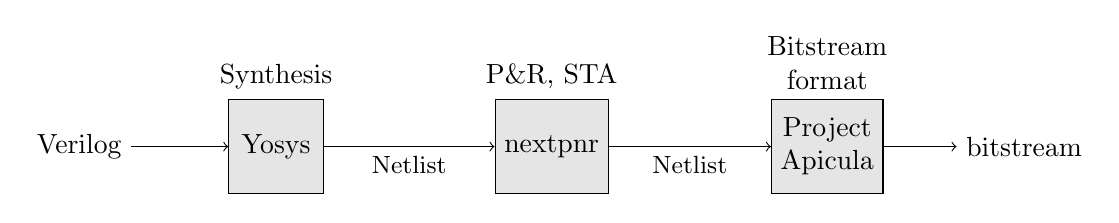
\begin{tikzpicture}[
  block/.style = {
    draw,
    shape=rectangle,
    minimum width=1.2cm,
    minimum height=1.2cm,
    fill=gray!20,
    align=center
  },
  %every path/.style={
  %  very thick,
  %  postaction={
  %    nomorepostaction,
  %    decorate,
  %    decoration={markings,mark=at position 0.5 with {\arrow{>}}}
  %  }
  %}
  %user/.style = {draw, shape=circle, inner sep=0, minimum size=2mm, align=center},
  %arrow/.style = {-Straight Barb},
]
  \node (verilog) {Verilog};
  \node (yosys)[
    right of=verilog,
    label=above:{Synthesis},
    block,
    xshift=15mm
  ] {Yosys};
  \node (nextpnr)[
    right of=yosys,
    %label=above:{P\&R},
    label=above:{\parbox[c]{3.0cm}{\centering P\&R, STA}},
    block,
    xshift=25mm
  ] {nextpnr};
  \node (apicula)[
    right of=nextpnr,
    label=above:{\parbox[c]{3.0cm}{\centering Bitstream\\format}},
    %label=above:{[align=center]Bitstream\\format},
    block,
    xshift=25mm,
    align=center
  ] {Project\\Apicula};
  \node (bitstream)[
    right of=apicula,
    xshift=15mm
  ] {bitstream};

  \draw[->] (verilog) -- (yosys);
  \draw[->] (yosys)   -- (nextpnr) node[below,midway] {\small Netlist};
  \draw[->] (nextpnr) -- (apicula) node[below,midway] {\small Netlist};
  \draw[->] (apicula) -- (bitstream);
\end{tikzpicture}

% \end{document}

  \end{center}
  \caption{EDA flow}
  \label{fig:eda-flow}
\end{figure}

\begin{table}
\centering
\begin{tabular}{lll}
  \toprule
  Tool           & Purpose                       & Version \\
  \midrule
  yosys          & Synthesis                     & 0.38    \\
  nextpnr        & Placement, routing, \gls{STA} & 0.7     \\
  Apycula        & Bitstream format handling     & 0.12    \\
  openFPGALoader & Loading design to FPGA        & 0.12.1  \\
  \bottomrule
\end{tabular}
\caption{Versions of software used for EDA}
\label{tab:tool-versions}  
\end{table}
